\documentclass[a4paper,11pt]{article}

\setlength{\parindent}{0mm}
\setlength{\oddsidemargin}{-5mm}
\setlength{\evensidemargin}{-5mm}
\setlength{\textwidth}{165mm}
\setlength{\textheight}{230mm}
\setlength{\topmargin}{-10mm}
\setlength{\marginparwidth}{15mm}
\setlength{\marginparsep}{7mm}
\usepackage{float}

%Include some packages which give certain fonts, graphics capabilities, etc
\usepackage{graphicx}% Include figure files
\usepackage{dcolumn}% Align table columns on decimal point
\usepackage{color}% bold math
\usepackage{bm}% bold math
\usepackage[caption=false]{subfig}
\usepackage{listings}





\begin{document}



% remove the following for publication
\begin{figure}
\leftline{\hfill The Zeeman Effect}
\end{figure}




% Front matter 
\title{An Investigation into the Charge mass Ratio of the Electron Using the Zeeman Effect and a Fabry–Pérot interferometer}
\author{Samuel Hedges}
\date{25/04/2022}
 \maketitle
 \newpage
\begin{abstract}
The Zeeman Effect and how it can be used in finding that charge mass ratio of an electron was looked into. It is found that to look at the charge mass ratio an Etalon is required. The Zeeman effect allows for the changing of the frequency of the wavelength, this changing that occurs due to the quantum exclusionary principle and magnetic moments, means that the released photons will take one of two components. The difference between these components can be measured. The charge mass ratio is correctly cited up to three significant figures as $(-2\pm0.3) \times10^{-11}$ $Ckg^{-1}$ which agrees with the given value of $-1.75 \times10^{-11}$ $Ckg^{-1}$ within one standard error. This shows that this experiment was successful in proving the theory and is accurate
\end{abstract}
 \newpage
 \tableofcontents
\newpage

\section{Introduction: Historical basis of Zeeman effect, Its Uses and the Charge Mass Ratio of the Electron}
The Zeeman effect is observed as the splitting of a spectral line into several components in the presence of a static magnetic field \cite{SCH1}. It was first observed in 1896 by Hendrik Lorentz and Peter Zeeman where they observed this splitting of spectral lines. They would go onto win the 1902 Nobel Prize for their work on the discovery of the effect.\\

The Zeeman effect can only be described through Quantum Mechanics. The effect implies that the component of angular momentum of an atom in the direction that is defined by an external magnetic field is quantized. The Magnetic moment means that it takes one of two results which is why the splitting is observed. This is counterfactual to Classical Mechanics where there are no discrete energy levels thus it is only described through Quantum Mechanics.\\

In this experiment the effect in cadmium is being observed due to it having a “normal” Zeeman effect. A normal Zeeman effect is a term coined for when there is zero net spin between certain energy levels of the atom \cite{SCH1}. The charge mass ratio of the Electron will be measured using its proportionality to a certain frequency shift as a result of the cadmium Zeeman effect.\\

 \begin{figure}[htb!]
       \centering
       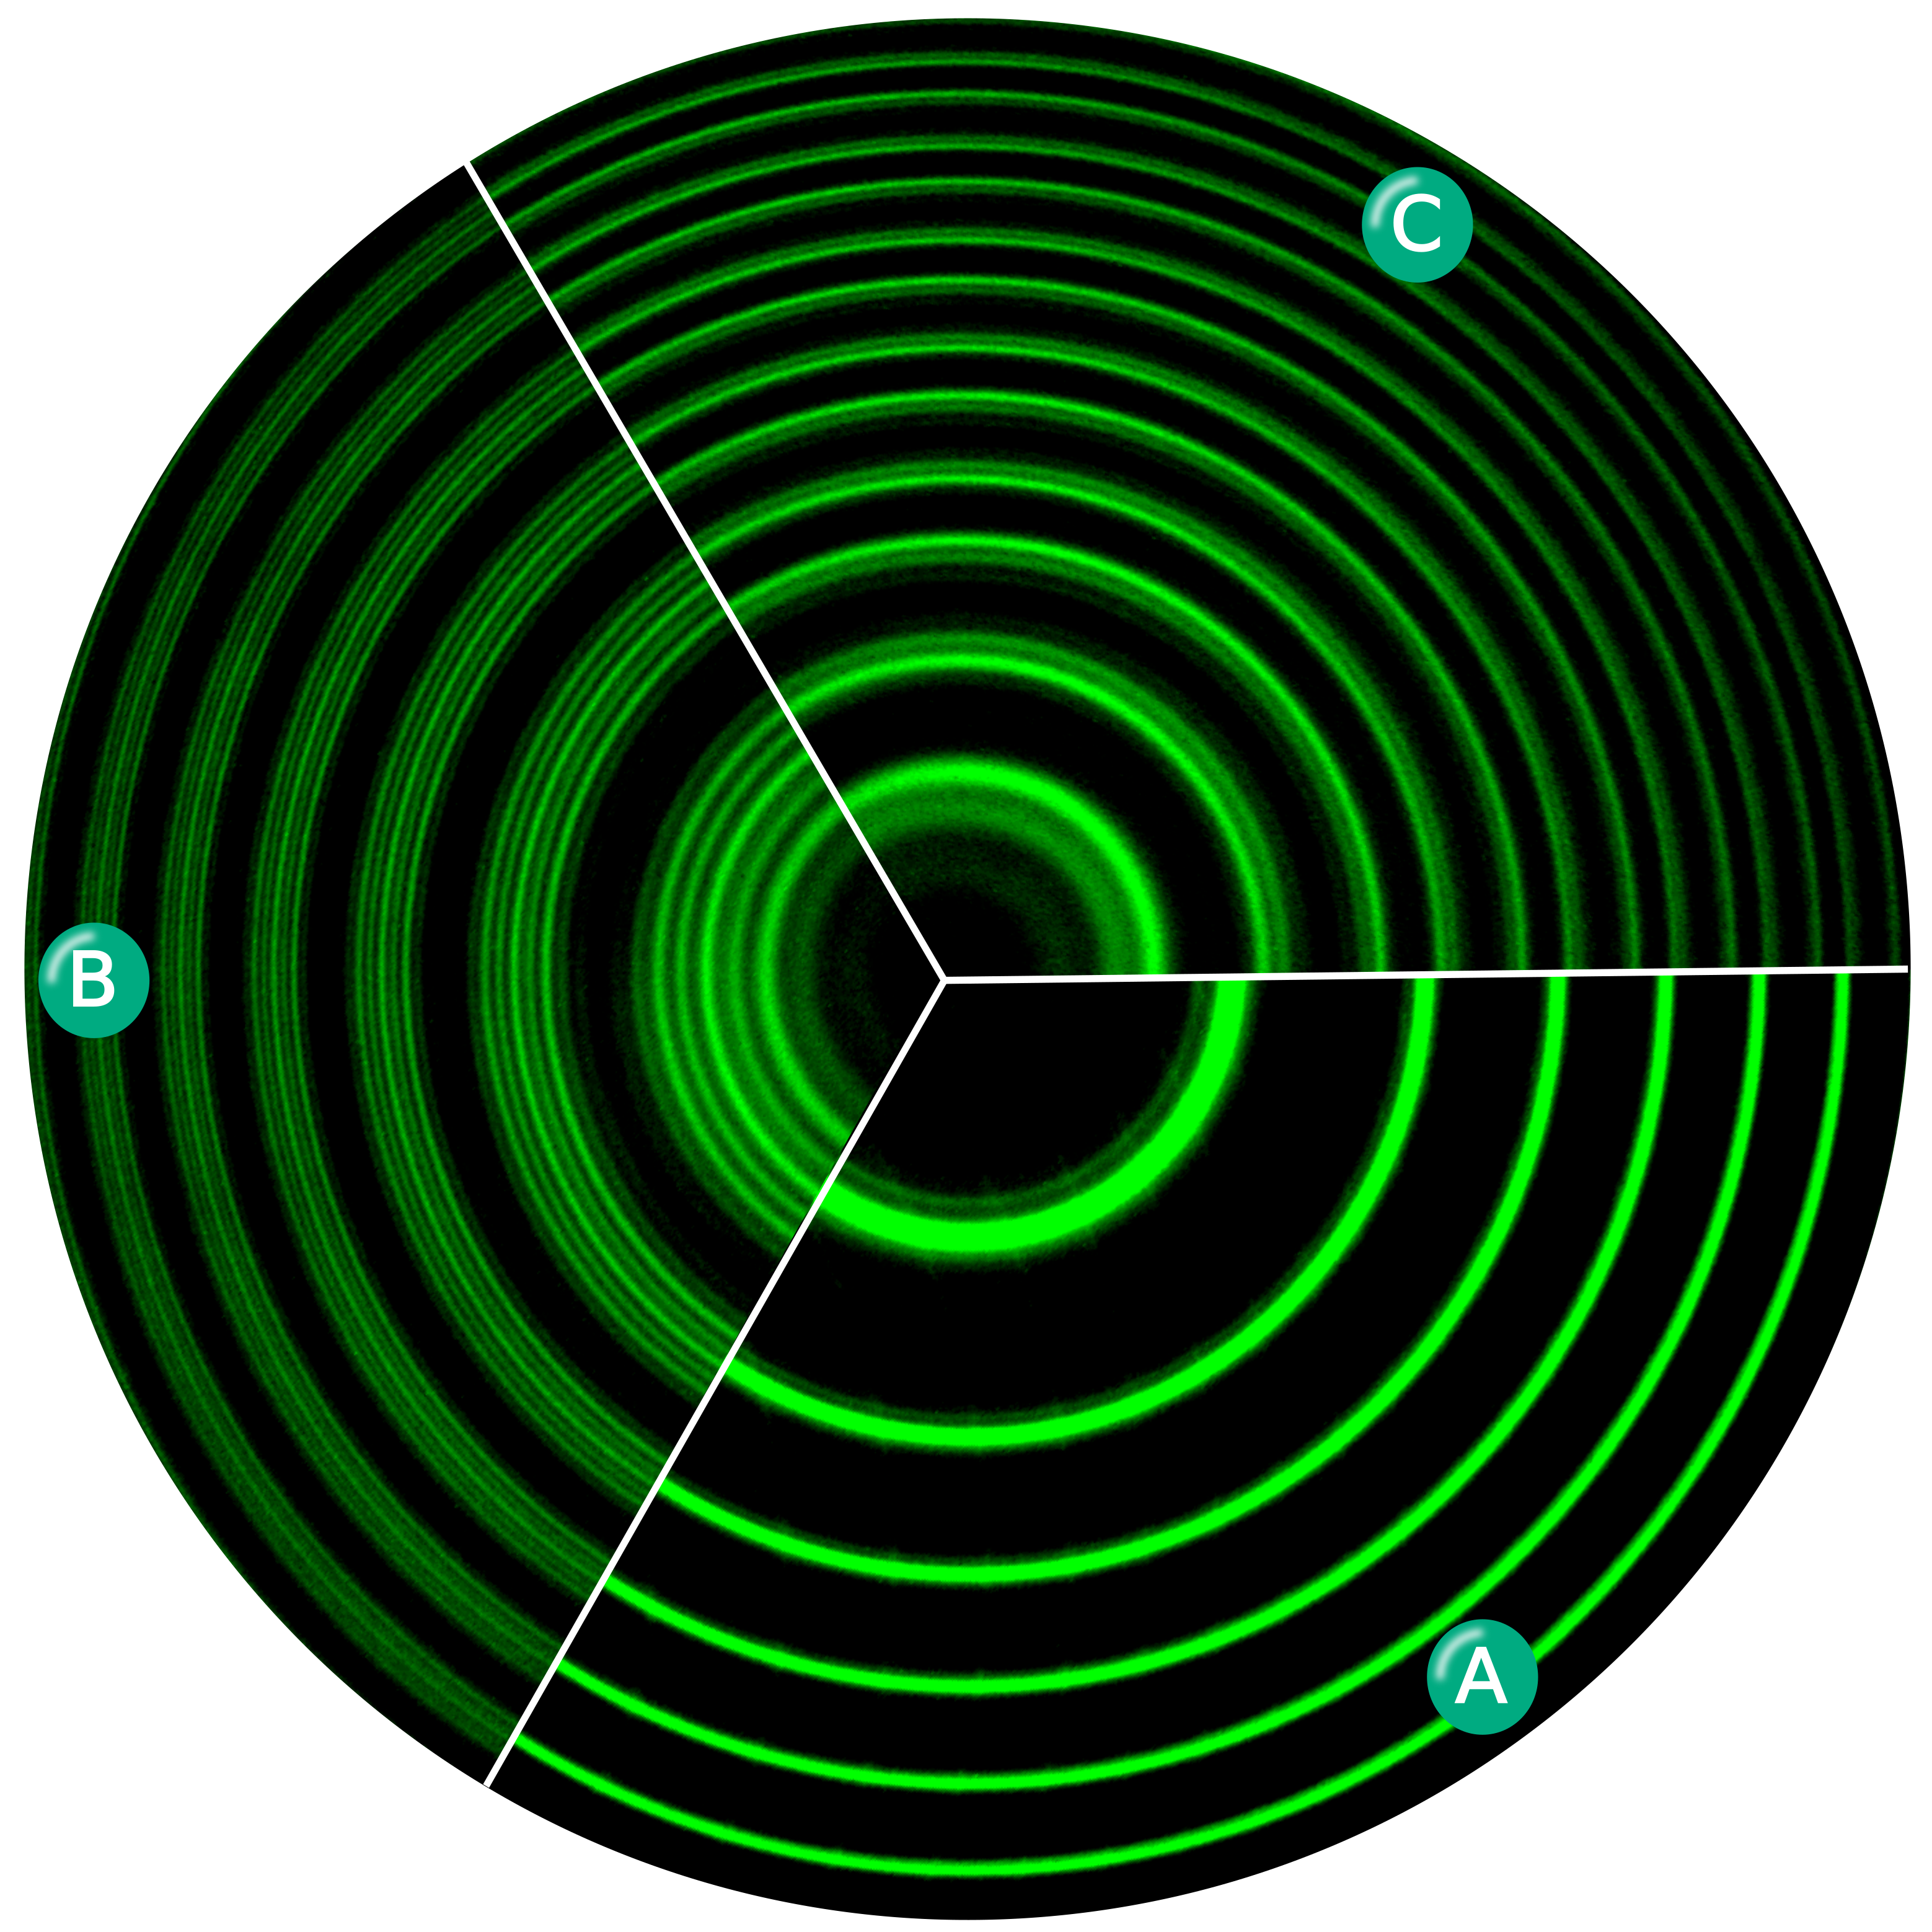
\includegraphics[width=0.4\columnwidth]{Images/Wiki Zeeman Effect.png}
        \caption{A Picture of an example of how the Zeeman effect changes the spectral lines of a mercury vapour lamp. Quadrant A shows the spectral lines without the Magnetic field, Quadrant B the magnetic field imposed over the atom \cite{Wikapidea Image 1}}
        \label{plot:Image of Zeeman Effect}
 \end{figure}

The Zeeman effect causes splitting that is proportional to the strength of the magnetic field used. This experiment used a Field strength typical for laboratories of roughly $6\times{10}^{-5}eV$ (Electron volts) which produced a splitting that was roughly ${10}^{-5}$ times the wavelength ($\lambda$) observed. The proportional nature of the Zeeman effect means that it is used to calculate the magnetic field strength of astronomical bodies like the sun. \cite{Zeeman Mag Fields} \cite{Star Zeeman}\\

The Zeeman effect is further used, and is applied, to technologies such as Nuclear Magnetic Resonance, Electron Spin Resonance, and Magnetic Resonance Imaging.\\

\section{Background Theory: How the Application of a Magnetic Field can cause the Zeeman} 

The Zeeman effect has a Quantum Mechanical explanation. From perturbation theory we can deduce the Hamiltonian 
\begin{equation}
    \hat{H}=\widehat{H_0}+V_M  \label{eq:Hamiltionian From Perturbation theory}
\end{equation}
Where $\widehat{H_0}$ is the unperturbed Hamiltonian and $V_M$ is the perturbation due to the magnetic field. This perturbation is the dot product between the magnetic moment of the atom and the Magnetic ($B$) field; 
\begin{equation}
V_M=-\vec{\mu_0}\cdot\ B \label{eq: Purtubation}
\end{equation}
\cite{Perturbed} The magnetic moment of an atom is given in terms of the total angular momentum vector $\vec{J}$ and the Lande “g-factor”. This g-factor comes about during the calculations of the first order perturbation in the energy of the atom. This results in the magnetic moment of the atom being: 
\begin{equation}
    \mu=\frac{-g_J\mu_B}{\hbar}\vec{J}\cdot\vec{B} \label{eq: The magnetic moment of an atom}
\end{equation}
If the Z-axis is defined along the path B enacts along, this dot product becomes: $\vec{J\ }\cdot\vec{B}=J_z\vec{B}$. Allowed spin values are defined as $m_J\hbar$ where the values of $m_J$ have been quantized such that they can only take the values ${-J, -J+1, …, +J}$. J is the total angular momentum quantum number. \\

From equation \ref{eq:Hamiltionian From Perturbation theory} it can be deduced that the change in energy is the same as this perturbation is given by 
\begin{equation}
    \Delta E=-g_J\mu_Bm_J \label{eq: Definition of CHnage in Energy}
\end{equation}
The transition that was being looked at in this experiment was the transition from a state $^1D_2\left(n=3\right)\rightarrow^1P_1(n=2)$ A, and since both states have a net-zero spin (known as a normal Zeeman effect), the total angular momentum is just equal to the orbital angular momentum. The $D_2$ state has five sub-states with a total angular momentum quantum number $J=L=2$, whereas the $P_1$ state has 3 sub-states and J=L=1. Since these are all spin zero sub-states, the “g-factor” is equal to 1, and they have equal separation of the sublevels. This shows that when there is a perturbation due to this magnetic field, that the $\Delta m_J=0$ or $\pm1$ which also follows from the fact that the emitted photon spin has a quantum number of 1. These three components will be called $\pi$ and $\sigma$ components, where $\pi$ components have 0 change in the angular momentum ($\Delta m_J=0$) and $\sigma$ components have an angular momentum: $\Delta m_J=\pm1$.\\

Knowing the change in energy in this process where there is a perturbation from the magnetic field, we can relate it to the frequencies to see the frequency shifts that will occur thanks to the imposition of the magnetic field over the cadmium light source. The Planck Relation states
\begin{equation}
    E=h\nu=\frac{hc}{\lambda} \label{eq: Planck's Relation}
\end{equation}
since both Planck’s constant and the speed of light are constants, the change in energy is: \begin{equation}
    \Delta E=hc\times\Delta(\frac{1}{\lambda})
\end{equation} \cite{Planck}. For $\pi$ components, there is no phase shift therefore $\Delta\left(\frac{1}{\lambda}\right)=0$. For the $\sigma$ components the phase change will be $\Delta\frac{1}{\lambda}=\pm\frac{e}{m}(\frac{B}{4\pi c})$. This shows that the electron charge mass ratio is calculated through observing the phase shift due to the Zeeman effect of a known magnetic field strength.\\

In this Experiment an electromagnet was being used. This meant that when calculating the Zeeman effect Magnetic Hysteresis had to be compensated for. Magnetic Hysteresis occurs when an external magnetic field is applied over a metal. The dipoles within the metal will then orientate themselves to the magnetic field. This alignment will cause the field strength to increase. This will affect the field strength and thus will affect our measurements for the Zeeman effect. To account for Magnetic Hysteresis, the magnetic field will be increased, then decreased. This will be done when both observing the Cadmium Effect and then with a magnetic field probe to allow for an accurate measurement of the magnetic field.\\

Due to the length of the wavelength, an etalon must be used to perceive the wavelength. An Etalon (or as it is otherwise known a Fabry-Perot Interferometer) is an optical cavity composed of two parallel surfaces made of a reflecting material. Optical rays are only able to pass through such a cavity if they are in resonance with the cavity. Due to constructive interference between different light launched into the mirrors depending on whether it is in phase, it will work to form a bigger image. This is detected by the two cameras allowing for measurements to take place. \cite{Etalon}
\begin{figure}[hbt!]
    \centering
    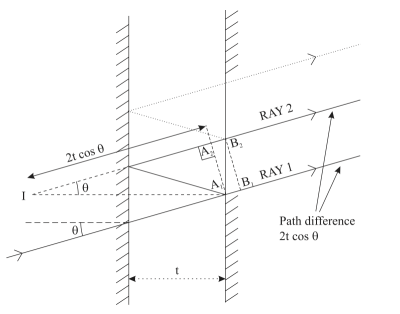
\includegraphics[width=0.5\columnwidth]{Images/tonk.png}
    \caption{This shows the wave diagram for an Etalon. This can be used to find the wavelength $lambda$ in terms of the Etalon opening} %YOU NEED TO QUOTE THE LAB MANUAL HERE!!!%
    \label{fig:my_label}
\end{figure}
 
 Through differentiation, we can find that the $$|\Delta \frac{1}{\lambda}|=|\frac{\Delta \lambda}{\lambda ^2}|=\frac{1}{2t}$$. This then means that if opening of the etalon is a known quantity, then the change in the wavelength of a wave passing though that Etalon can be found. 

\section{Apparatus and Experiment: The Set-up and Components of the Optical Bench and Cadmium Light Source }

\subsection{Components used}
The Equipment and set-up used in this experiment can be seen in Figure \ref{fig:Experimental Set-up}
\begin{figure}[htb!]
    \centering
    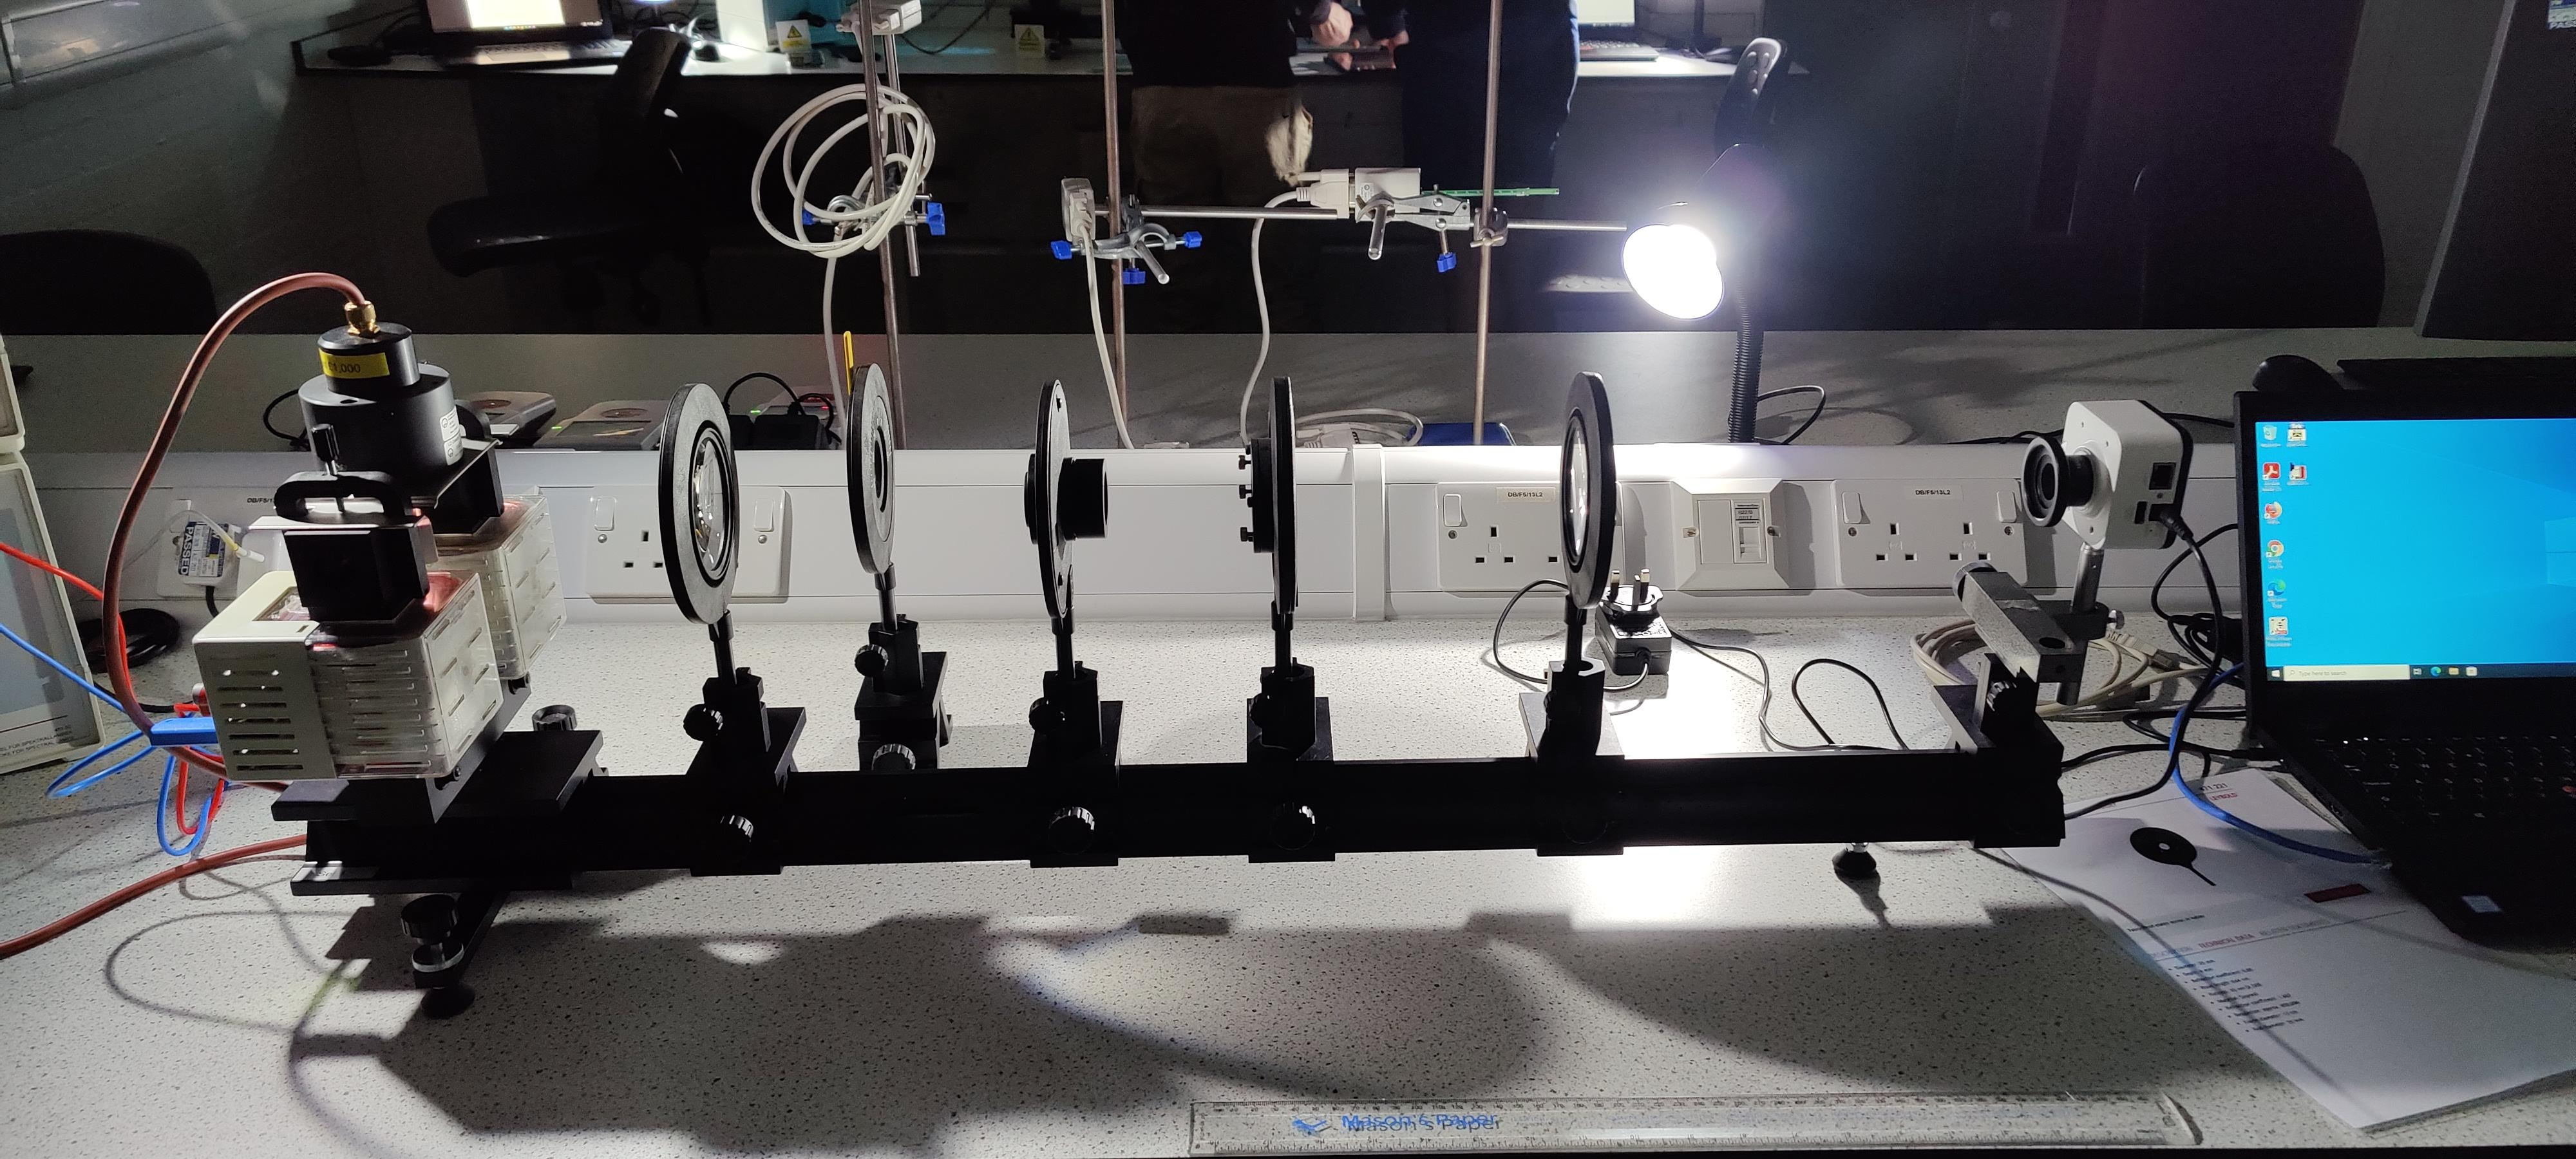
\includegraphics[width=0.9\columnwidth]{Images/Cadmium Zeeman Set-up 3.jpg}
    \caption{A picture of the set-up used to take measurements for the Zeeman Effect in Cadmium. At the left of the image is the Cadmium light source with the electromagnet over. The next instrument on the optical bench is the diverging lens. The red filter is the next instrument then the Etalon. then finally the converging lens and camera}
    \label{fig:Experimental Set-up}
\end{figure}

In this set up the first diverging lens was used to diverge the light, so it could be converged onto the camera by the second lens, and thus create an image. The red filter was just to focus on the specific colour of light for the specific transition being observed. The Etalon as discussed in the theory section is increasing the size of the image, so it can be observed. The Camera on the end was replaced with a CCD linear optical array whilst the measurements were being taken


\subsection{Method}
To achieve the Set-up seen in Figure \ref{fig:Experimental Set-up} an optical camera was used. the two lenses were adjusted on the optical bench till a clear image was observed on the computer screen. When this occurred it meant that the lenses were focused.
\begin{figure}[hbt!]
    \centering
    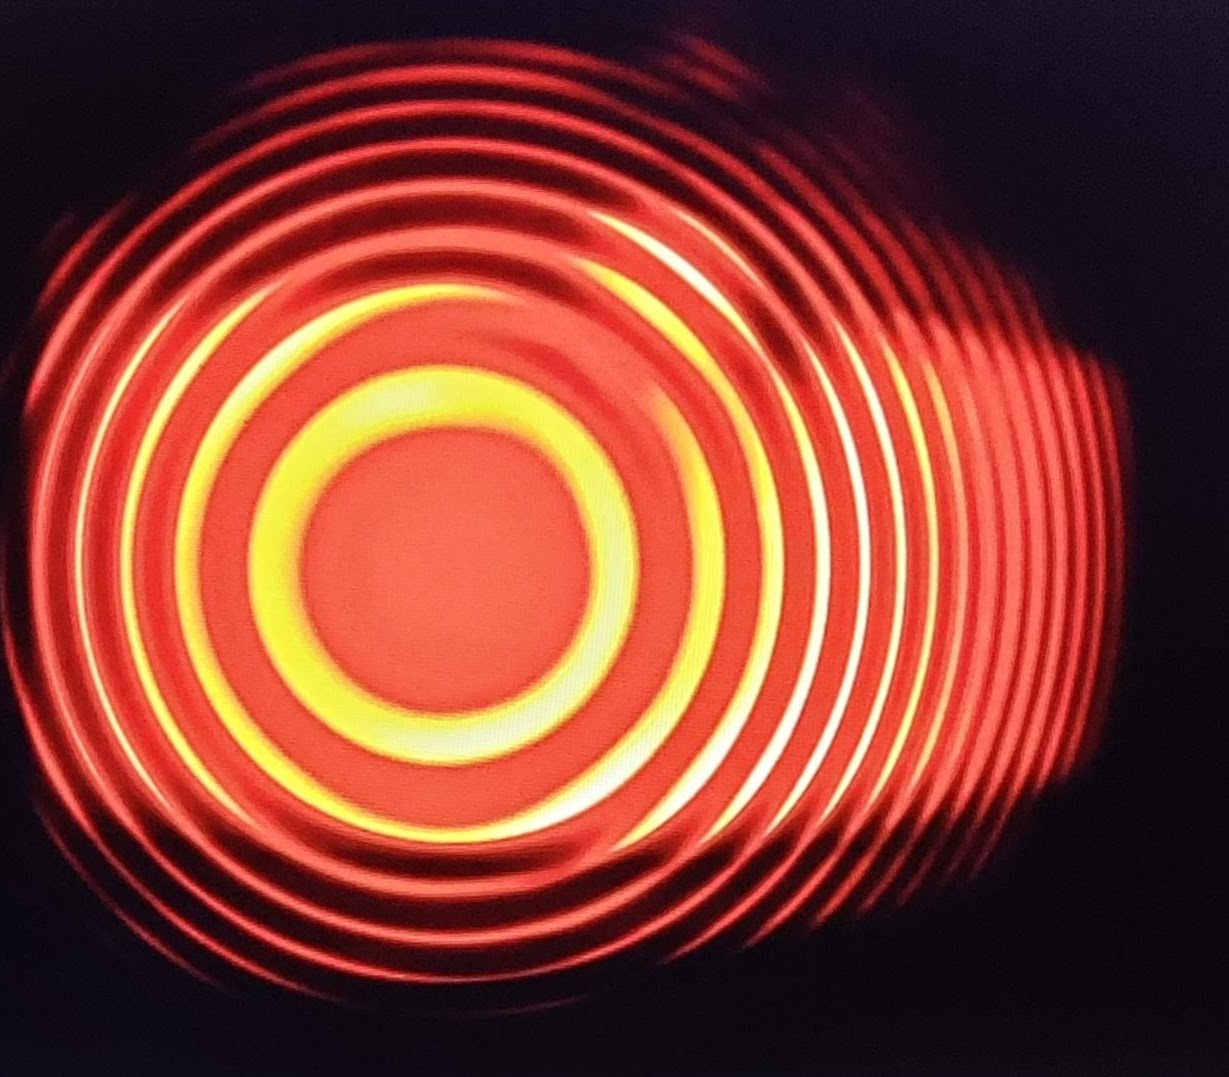
\includegraphics[width=0.2\columnwidth]{Images/Waveform Pic.jpg}
    \caption{This image was captured by the optical camera once the lenses were aligned. It shows the cadmium waveform produced from the Etalon (The Zeeman effect was not being observed at this point as the electromagnet was not on)}
    \label{fig:Picture of the image}
\end{figure}

The CCD linear optical array was then switched out for the optical camera. The array was then adjusted till the maximum peaks were observed. The electromagnet was then switched on and the Zeeman Effect was observed. Measurements were taken with the linear array using the graph produced. To account for the magnetic hysteresis these measurements were taken from zero increasing to 7 amps (over the electromagnet) Then decreasing it to 0 amps (over the electromagnet) once more.\\

The splitting caused to the Wavefronts observed by the CCD linear array was noted (measuring from the central $\pi$ peak to the two smaller $\sigma$ peak).\\

To find the Magnetic field strength at the current, the electromagnet was increased and decreased again this time with a magnetic field probe measuring the magnetic field. This gave us an uncertainty for the magnetic field at a given current which could be used to find the electron charge mass ratio.
\section{Results & Analysis: The Outcome of the Charge Mass Ratio of The Electron and How the Magnetic Hysteresis was Accounted For}
The Zeeman Effect was Observed 5 times. An Average of the five can be found in table \ref{tab:I hate Myself}
\begin{table}[hbt!]
    \centering
    \begin{tabular}{|c|c|c|c|}
    \hline
       Current Over the & Mean difference in the & Standard Deviation in the  & Uncertainty in the \\
         electromagnet & $\pi$ and $\sigma$ components & Difference of the $\pi$ and $\sigma$ components & Difference in \\
         (Amps) & (Pixels) & (Pixels) & the split peaks \\
         \hline\hline
         $\uparrow$ 5.0 & 13.75 & 0.5 & 1.414214\\
         $\uparrow$ 5.2 & 14.5 & 0 & 1.414214\\
         $\uparrow$ 5.4 & 14.75 & 0.288675 & 1.414214\\
         $\uparrow$ 5.6 & 15.5 & 0 & 1.414214\\
         $\uparrow$ 5.8 & 15.5 & 0 & 1.414214\\
         $\uparrow$ 6.0 & 15.875 & 0.25 & 1.414214\\
         $\uparrow$ 6.2 & 16.25 & 0.288675 & 1.414214\\
         $\uparrow$ 6.4 & 16.5 & 0 & 1.414214\\
         $\uparrow$ 6.6 & 16.75 & 0.288675 & 1.414214\\
         $\uparrow$ 6.8 & 17.25 & 0.288675 & 1.414214\\
         $-$ 7.0 & 17.5 & 0 & 1.414214\\
         $\downarrow$ 6.0 & 16.375 & 0.25 & 1.414214\\
         $\downarrow$ 5.0 & 13.875 & 0.25 & 1.414214\\
         $\downarrow$ 4.0 & 11.375 & 0.25 & 1.414214\\
         $\downarrow$ 3.0 & 8.75 & 0.288675 & 1.414214\\
         $\downarrow$ 2.0 & 5.5 & 0 & 1.414214\\
         $\downarrow$ 1.0 & 1.5 & 0.408248 & 1.414214\\
         $\downarrow$ 0.0 & 0.0 & 0 & 1.414214\\
         \hline
    \end{tabular}
    \caption{The results from the averaging of four repeated measurements of the difference in peaks from the $\pi$ components and the $\sigma$ components. The arrows represent whether the current is increasing or decreasing}
    \label{tab:I hate Myself}
\end{table}

The statistical Uncertainty was smaller than what would be expected from random error, therefore, the uncertainty of $\pm 1$ was used for the uncertainty to account for the random uncertainty. This table will allow for the calculation of the charge mass ratio of the Electron\\

\begin{table}[hbt!]
    \centering
    \begin{tabular}{|c|c|c|}
    \hline
         Current over & Magnetic Field & ratio of the\\
          electromagnet & Strength & spectral range \\
          (amps) & (Tesla) & \\
    \hline\hline
         $\uparrow$ 5.0 & 0.457 & 0.232264 \\
         $\uparrow$ 5.2 & 0.48 & 0.244932\\
         $\uparrow$ 5.4 & 0.488 & 0.249155\\
         $\uparrow$ 5.6 & 0.488 & 0.261824\\
         $\uparrow$ 5.8 & 0.511 & 0.261824\\
         $\uparrow$ 6.0 & 0.521 & 0.268159\\
         $\uparrow$ 6.2 & 0.531 & 0.274493\\
         $\uparrow$ 6.4 & 0.543 & 0.278716\\
         $\uparrow$ 6.6 & 0.551 & 0.282939\\
         $\uparrow$ 6.8 & 0.561 & 0.291385\\
         $-$ 7.0 & 0.567 & 0.295608\\
         $\downarrow$ 6.0 & 0.529 & 0.276605\\
         $\downarrow$ 5.0 & 0.467 & 0.234375\\
         $\downarrow$ 4.0 & 0.376 & 0.192145\\
         $\downarrow$ 3.0 & 0.281 & 0.147804\\
         $\downarrow$ 2.0 & 0.19 & 0.092905\\
         $\downarrow$ 1.0 & 0.0953 & 0.025338\\
         $\downarrow$ 0.0 & 0.00064 & 0\\
         \hline
    \end{tabular}
    \caption{This is the results from the magnet probe when investigating the magnetic field strength of the electromagnet. We can use this to find the charge mass ratio of the electron. The arrows show whether the current was increasing or decreasing}
    \label{tab:Why are we still here?}
\end{table}

From Table 1 and 2, a graph can be drawn to find the charge mass ratio of the electron through plotting a graph of the ratio of f to 2t against the magnetic field strength divided by $4\pi$ times the speed of light.
\begin{figure}[hbt!]
    \centering
    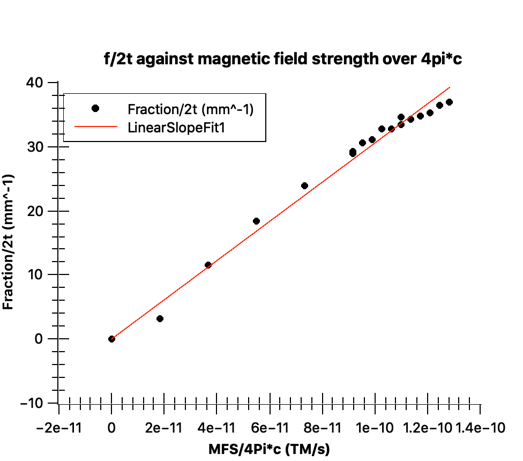
\includegraphics[width=0.35\columnwidth]{Images/Pic for Lab I Guess.png}
    \caption{This is the plot of the $\frac{f}{2t}$ against $\frac{B}{4\pi c}$. From the gradient of this graph the charge mass ratio of the Electron was found to be $(-2\pm0.3) \times10^{-11}$ $Ckg^{-1}$}
    \label{fig:Final Graph}
\end{figure}

The electron charge mass ratio from this experiment, as stated, was found to be $(-2\pm0.3) \times10^{-11}$ $Ckg^{-1}$. The given charge mass ratio of the electron can be cited to be $-1.75 \times10^{-11}$ $Ckg^{-1}$ \cite{Electron}. Since our value agrees with the given value within one standard deviation it can be said that our experiment has shown to be reproducible as it has been corroborated by different groups using different equipments. Since this value is also corroborated by other groups on the same experiment we can also say that this experiment is repeatable. The experiment agreeing with the given value also shows that the experiment was accurate, the fact that the uncertainty in this value was relatively low shows that the experiment was also precise

\section{Conclusion: If Calculating the Charge Mass Ratio of the Electron From the Zeeman Effect can be done}
This experiment was undertaken so that we could observe the Zeeman effect and the changes it caused as well as understanding the Etalon better. This experiment was also undertaken to find the charge mass ratio of the electron.\\

In this experiment it has been shown that the charge mass ratio of an electron can be found by observing the shift in the Frequency of light produced, caused by the normal Zeeman Effect in cadmium seen through the diffraction in an Elton. The value recovered for the charge mass ratio of the electron was $(-2\pm0.3) \times10^{-11}$ $Ckg^{-1}$, and the given value is $-1.75 \times10^{-11}$ $Ckg^{-1}$ \cite{Electron} which is within a standard error of the given value and therefore we have shown that this experiment is precise and accurate.\\

The clear agreement between the results of this experiment and the supporting theory further goes to show that the use of the Zeeman effect and knowledge of it was correct. The use of a net-zero spin between the states for the cadmium light source has been shown to be an accurate measurement. This helps further the understanding of how quantum effects can be used to describe subatomic \\

This experiment could have been improved by a number of changes. As can be seen in figure \ref{fig:Experimental Set-up}, the equipment was not perfectly level (aligned in the horizontal direction. this caused the waveform on the screen to be slightly off and thus made measurements harder to take. This may have caused an error when looking at some differences in the peaks for $\pi$ and $\sigma$ components and thus may also have offset the measurements.
Taking more measurements with the magnetic field probe would have also made the experiment more precise. In this experiment the magnetic field was only measured twice, meaning that not much of an average or standard error could be calculated from the values.\\

During this experiment there were safety precautions followed to keep the equipment and those undertaking the experiment safe. The electromagnet gets hot during prolonged use therefore a current was not passed over it continuously for more than 5 minutes. Handling the electromagnet did not happen unless it had been kept off for more than 20 minutes so that there would be no burns. All the equipment was also fixed to the optical bench to prevent any damage to the equipment and any risk of injury linked will poorly fixed equipment.\\


\newpage
\section{Bibliography}
\begin{thebibliography}{}
    \bibitem{Wikapidea Image 1} By Warren Leywon - Own work, CC BY-SA 4.0, https://commons.wikimedia.org/w/index.php?curid=65502984
    
    \bibitem{SCH1}Sutter DH, Flygare WH. The molecular Zeeman effect. InBonding+Structure 1976 (pp. 89-196). Springer, Berlin, Heidelberg.
    
    \bibitem{Zeeman Mag Fields}Shulyak D, Reiners A, Engeln A, Malo L, Yadav R, Morin J, Kochukhov O. Strong dipole magnetic fields in fast rotating fully convective stars. Nature Astronomy. 2017 Jul 24;1(8):1-7.
    
    \bibitem{Star Zeeman}Babcock HW. Zeeman Effect in Stellar Spectra. The Astrophysical Journal. 1947 Jan;105:105.
    
    \bibitem{Perturbed}Iliopoulos J, Itzykson C, Martin A. Functional methods and perturbation theory. Reviews of Modern Physics. 1975 Jan 1;47(1):165.
    
    \bibitem{Planck}Bose SN. Planck's law and the light quantum hypothesis. Journal of Astrophysics and Astronomy. 1994 Mar;15:3.
    
    \bibitem{Etalon}Reardon KP, Cavallini F. Characterization of Fabry-Perot interferometers and multi-etalon transmission profiles-The IBIS instrumental profile. Astronomy & Astrophysics. 2008 Apr 1;481(3):897-912.

    \bibitem{Electron}Gräff G, Kalinowsky H, Traut J. A direct determination of the proton electron mass ratio. Zeitschrift für Physik A Atoms and Nuclei. 1980 Mar;297(1):35-9.
\end{thebibliography}

\end{document}